\documentclass[letterpaper]{article}
\usepackage[backend=biber,style=authoryear,citestyle=authoryear]{biblatex}
\addbibresource{./mybib.bib} %biblatex
\usepackage{alifeconf}
\usepackage{url}
\def\code#1{\texttt{#1}} % shortcut for monospaced

% Tables
\usepackage{array}
\usepackage{booktabs}
\usepackage{colortbl}

\title{Speech-To-Text Engine for Forced Alignment}
\author{Daniel Tiefenauer (daniel.tiefenauer@students.fhnw.ch)\\
\mbox{}\\
Institute for Data Science (I4DS), University of Applied Sciences FHNW, Windisch (Switzerland)}

\pagestyle{plain}

\begin{document}	
\maketitle

\begin{abstract}
\textit{Forced Alignment} is concerned with aligning chunks of text (e.g. parts from a transcript) with parts of a corresponding audio signal. This involves enriching the textual data with temporal data. The process is usually very time consuming because it is often done by hand. This paper introduces an method that reduces said time by producing alignments automatically. The result can be used as-is or with little manual adjustments. The method uses a pipeline which automatically detects voiced segments, transcribes them and aligns the partial transcript with the full transcript using Global Sequence Alignment. Transcriptions are produced by a \textit{Speech-To-Text (STT)} engine building upon simplified architecture of the \textit{DeepSpeech} architecture. The main idea beind this is that Global Alignment can be done even if the partial transcripts match the ground truth only poorly. It has been shown that such transcripts can be obtained from a STT engine trained on very little training data.
\end{abstract}

\section{Introduction}
\textit{Automatic Speech Recognition (ASR)} has made huge progress in recent years. One idea that had a significant impact on ASR was \textit{Connectionist Temporal Classification (CTC)} \parencite{ctc_paper}, which can be used in \textit{Sequence-to-Sequence (S2S)} models and produces an output sequence of labels for an input sequence of features. CTC is often used in STT engines where the input sequences are audio features (e.g. spectrograms) and the output sequences are their transcripts (i.e. a sequence of characters). Such engines use probabilistic models whereas for each input frame a distribution over the output labels is calculated. The input sequence is typically much longer than the output sequence. The advantage of CTC is that it is \textit{alignment-free}. The optimal alignment is found by calculating the probabilities of each alignments using dynamic programming and then marginalizing over the set of valid alignments (alignments collapsing to the actual transcription). 

A famous architecture for a S2S model using CTC has been proposed by \textit{DeepSpeech} \parencite{deepspeech}. A slightly modified implementation is continuously being developed by Mozilla\footnote{\url{https://github.com/mozilla/DeepSpeech}}, achieving \textit{Word Error Rates (WER)} of as low as 6.5\% \parencite{mozillajourney}. One approach for \textit{Forced Alignment} could now be to simply transcribe the audio and run some sort of spell-checker over the result in order to get the full transcript. However, such a transcript would then include unwanted effects like stuttering, repetitions, mispronunciation etc. Another approach would be to align the produced transcript with a known ground truth. However, this is only possible for languages where a STT engine is readily available. This is often not the case for minority languages like Swiss German. Training an ASR model for those language usually requires large amounts of training data which are often not available.

This paper focuses on aligning chunks of text, not individual characters. It draws upon the assumption that for this purpose a STT engine producing only very low-quality transcripts might be sufficient. Such inferior transcripts can still be good enough for a Sequence Alignment algorithm which aligns them with some sort of ground truth. A fully-fletched STT engine like the one provided by Mozilla on the other hand are targeted at high recognition rates. This quality is probably not needed in the first place. 

This paper therefore uses a simplified version of the \textit{DeepSpeech} model as implemented by Mozilla, which uses a \textit{Recurrent Neural Network (RNN)} with CTC as its cost function. The main idea behind this is that a simpler model requires significantly less data than a sophisticated variant and can therefore be trained for languages where such data might be scarce.

\section{The pipeline approach}

This paper introduces a pipelined approach for automated \textit{Forced Alignment}. A combination of audio (the \textit{signal}) and text (the \textit{ground truth}) can be put through this pipeline, resulting in a list of aligned text passages. Each item in this list contains the desired temporal information (i.e. start and end frame in the audio signal) as well as the partial transcript that lead to the alignment. The pipeline consists of four stages:

\begin{enumerate}
	\item \textit{Preprocessing}: Preparing the signal and ground truth for inference resp. for training
	\item \textit{Voice Activity Detection (VAD)}: Splitting the audio signal into voiced segments
	\item \textit{Automatic Speech Recognition (ASR)}: Transcribing each voiced segment
	\item \textit{Global Sequence Alignment (GSA)}: Aligning each partial transcript with the ground truth
\end{enumerate}

All stages were implemented in Python. Since the GSA stage operates on character level, a low \textit{Label Error Rate (LER)} is desireable. The key stage for this is the STT engine in the ASR stage because -- although being simple and trained on little data -- it should be able to produce \textit{good enough} transcripts fit for the downstream GSA stage.

\subsection{Preprocessing}

Since the model architecture is based on the Mozilla implementation of \textit{DeepSpeech}, the input data must be transformed to a compatible format. Audio signals are converted to mono PCM-16 wave files encoded with 16-bit raw bytes (little-endian). The text data is normalized by restricting it to an alphabet used by the corresponding language. Such an alphabet usually consists of the letters of the latin alphabet as well as other characters commonly found in the language (like the apostrophe in English or umlauts in German). Normalization is done by lowercasing the text and removing punctuation.

\subsection{Voice Activity Detection (VAD)}

The preprocessed audio signal is split into non-silent parts by using the Python port\footnote{\url{https://github.com/wiseman/py-webrtcvad}} of the \textit{WebRTC} project\footnote{\url{https://webrtc.org}}. This algorithm has proved to be very efficient both in time needed to make the split as well as in the quality of the splits.

\subsection{Automatic Speech Recognition (ASR)}

The STT model is implemented using the \textit{Keras} framework and is based on the Mozilla implementation of \textit{DeepSpeech}. The Mozilla architecture was simplified by not using a Language Model (LM) in the training process, discarding the convolution in the first layer and not using context frames. The model uses a sequence of $T_x$ MFCC features with $n=26$ features in its input layer. The input is put through three fully connected layers with 1,024 units followed by a bidirectional layer. All intermediate layers use LSTM cells with 1,024 units and the \textit{Rectified Linear Units (ReLU)} activation function because this has been proved to work well for acoustic models \parencite{relu}. The output layer is again fully-connected using softmax to produce a vector of probabilities for each feature vector. Experiments were made with and without regularizing the model using dropouts between each layer. The LER and WER on the validation set was slightly lower with the regularized model. Figure \ref{model_architecture} shows the simplified model graph.

\begin{figure}[!htb]
	\begin{center}
		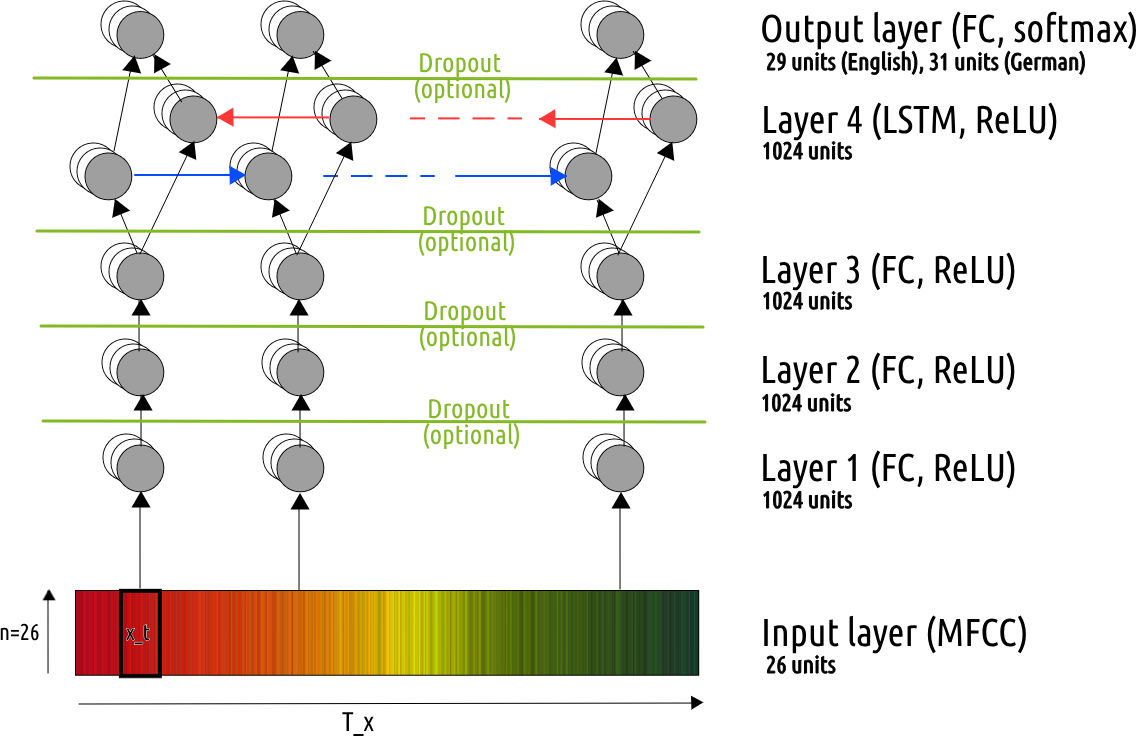
\includegraphics[width=3.5in]{model_architecture.png}
		\caption{Simplified RNN architecture proposed in this paper. Each input frame $t_x$ in the $(n \times T_x)$ input layer is put through a series of fully-connected (FC) layers. Layer 4 is a bidirectional recurrent layer. The output layer assigns a probability distribution for each input frame.}
		\label{model_architecture}
	\end{center}
\end{figure}

\subsection{Global Sequence Alignment (GSA)}

The partial transcripts produced by the ASR stage are concatenated and separated by a single space to a string $B$ . This string is then aligned with the full transcript as reference string $A$. A modified version of the \textit{Needleman-Wunsch} algorithm is used for global alignment. This algorithm calculates a matrix of alignment costs and then backtracks it to find the optimal alignment for characters of string $B$ with string $A$ by dropping or inserting characters.

Because in its original form, the \textit{Needleman-Wunsch} algorithm has no notion of partial transcripts it does not keep track of where they start and end. The modified algorithm therefore produces a list of alignments by annotating the string of concatenated partial transcripts with information about the boundaries of the partial transcripts. Because the optimal alignment is found by tracing the cost matrix from the back, the end index $j_{end}$ of a partial transcript is encountered before its starting index $j_{start}$. Each time an end $j_{end}$ index is aligned with some index $i_{end}$ in the reference string, this index is noted. As soon as the start index $j_{start}$ is encountered, the corresponding start index $i_{start}$ in the reference string is also noted. The aligned text for the partial transcript can then be created by extracting the substring $A[i_{start} : i_{end}]$ from the reference string.

\section{Training the simplified model}

Two different variants of the simplified model were trained to recognize German and English. For the English variant the output layer consisted of 29 units because the probability was calculated for 29 labels\footnote{26 lowercase letters from the alphabet, space, apostrophe and the blank token used by CTC}. Because the apostrophe is far less common in German, this character was dropped for the German variant. Instead, umlauts were added to the set of labels because they are very common in German. Therefore the German model used 31 units in its output layer\footnote{26 lowercase letters from the alphabet, 3 umlauts, space, blank token}. Both variants were regularized by adding dropouts between the layers.

\subsection{English model variant}
The English variant of the simplified model was trained on the \textit{CommonVoice (CV)} corpus, which is built and maintained by Mozilla\footnote{\url{https://voice.mozilla.org}} and is also used to create a pre-trained model using Mozilla implementation of \textit{DeepSpeech}\footnote{\url{https://github.com/mozilla/DeepSpeech#getting-the-pre-trained-model}}. The samples from the training set were sorted by their audio length. Only the first 1,000 minutes of audio were used for training. The CTC training loss was calculated for these samples. Samples from the validation set were used to calculate the validation loss. Figure \ref{loss_en} shows the curve for both losses. It is evident that the model does not improve anymore after epoch 15 and start to overfit after that.

\begin{figure}[!htb]
	\begin{center}
		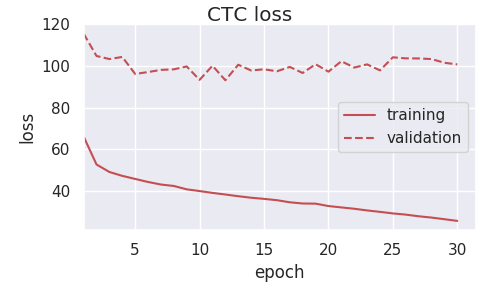
\includegraphics[width=3.5in]{loss_en.png}
		\caption{Plot of the CTC loss for training and validation data. Because the validation loss does not decrease after epoch 15, the model will start to overfit after that point.}
		\label{loss_en}
	\end{center}
\end{figure}

Additionally, the model was used after each epoch to make inferences on the samples from the validation set using \textit{Beam Search Decoding} \parencite{ctc_paper}. Each inference was compared against its ground truth by calculating the LER. Figure \ref{ler_en} shows how this metric evolves with the training progress.

\begin{figure}[!htb]
	\begin{center}
		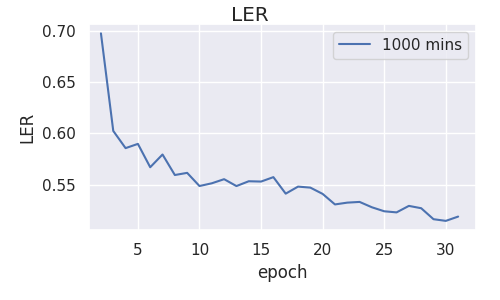
\includegraphics[width=3.5in]{ler_en.png}
		\caption{Plot of the average LER between inference and ground truth. The inferences were made for samples from the validation set using the model trained on 1,000 minutes of data from the CV corpus after each.}
		\label{ler_en}
	\end{center}
\end{figure}

\subsection{German model variant}

For the German variant of the simplified model labelled data with a total audio length of approximately two hours was used. This data consists of recordings of German speakers and their transcripts. The split into training-, validation- and test-set was done automatically and not with the same diligence as the CV corpus meaning the distribution of sexes, accents etc. might not reflect a realistic setting. The split was done so the training set contained 80\% of the labelled data and the validation and test set 10\% each. The training set hence contained only about 80 minutes of audio data which were augmented by adding distortion (change of pitch, tempo or volume and adding delay or echo). Each of these distortions was applied in isolation and combination until 1,000 minutes of audio data were available. Training was then done like with the English variant. Figure \ref{loss_de} shows the progress of the training loss.

\begin{figure}[!htb]
	\begin{center}
		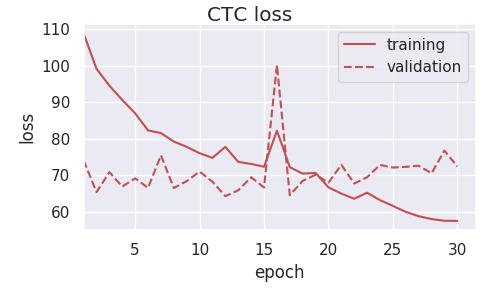
\includegraphics[width=3in]{loss_de.png}
		\caption{Plot of CTC training- and validation- loss when training on German samples. 1000 minutes of original and synthesized data were used. There is an inexplicable spike at epoch 16.}
		\label{loss_de}
	\end{center}
\end{figure}

Apart from an awkward spike in epoch 16 the plot is similar to the one from the English variant in that there is a slight trend to increasing validation loss after epoch 15. Figure \ref{ler_de} shows the progress of the LER on validation data.

\begin{figure}[!htb]
	\begin{center}
		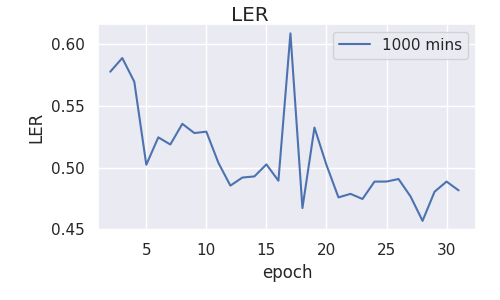
\includegraphics[width=3in]{ler_de.png}
		\caption{Curve of the LER when calculated for inferences from the validation set. Note the spike in epoch 16 is also visible here.}
		\label{ler_de}
	\end{center}
\end{figure}

The trend for the LER is less smooth than with the English model. The spike from the CTC-loss is also visibile here.

\section{Using a simple spell-checker}

Since the simplified model produces a transcript as an arbitrary sequence of characters, experiments were made whether these results could be improved by applying some sort of spell checking. For this a simple spell-checker was implemented that uses a vocabulary $V$ of the 80,000 most frequent word of the corpus it was trained on. The space separated word tokens from the inference were compared against this vocabulary. If the word token appeared in the vocabulary it was deemed valid and the next word was compared. If it did not appear in the vocabulary, all variants of the word with edit distance 1 were created by adding, removing or changing individual characters in the word with characters from the alphabet. Only the set $W_1$  of variants that appeared in the vocabulary were kept. If this set was empty ($W_1 = \emptyset$), the set $W_2$ of variants with edit distance 2 was created from $W_1$ similarly. If $W_2 = \emptyset$ the unchanged original word was kept. 

All word tokens from an inference were processed from left to right with above procedure. Partial sentences were created by producing the cartesian product of all combinations. After each word the likelihood of each partial sentences was estimated using a 5-gram \textit{Language Model (LM)} and only the 1,024 most likely combinations were kept. After all words were processed, the most likely sentence was kept as the corrected sentence.

For English, the \textit{KenLM} ·\parencite{kenlm} model available from the pre-trained model from Mozilla was used to make the estimation. For German a custom model was trained on a text corpus derived from about 2.2M Wikipedia articles. The articles were normalized by removing Wiki markup, lowercasing the text and tokenizing the text into lines of individual sentences. Furthermore, numeric tokens were replaced by the \code{<num>} token because such tokens represent values (e.g. year numbers) and do not carry semantic meaning.

With above procedure a rudimentary spell-checker was implemented. Although some informal experiments showed the spell-checker is working provided the LER is sufficiently low, it did not improve the inferences produced by the simplified model in most cases. Often the corrected inference had a higher LER than the original inference when compared to the ground truth because the character sequences were changed to a wrong word. Apparently the LER of the original inference is still too high for such a spell checker. Therefore the original uncorrected inferences were used for the GSA stage.

\section{Tests and results for English samples}

The alignments produced by the pipeline using the simplified model were evaluated by comparing them against alignments produced the same pipeline but using the pre-trained model from Mozilla as a reference model in the ASR stage. The test set consisted of audio and text samples from the \textit{LibriSpeech} corpus\footnote{\url{http://www.openslr.org/12/}}. This corpus contains speech samples from recordings of books read by various speakers. Audio and text data were derived by exploiting the corpus metadata. The audio files were created on a per-speaker basis by cropping the original recordings so that the signal begins with the first sample from the corpus entry and ends with the last sample. The transcript was extracted by looking up the transcript of the first and the last speech sample in the original book text. Some of the transcripts had to be manually adjusted to make sure they only contain the spoken text for each recording. Both audio and text were preprocessed as described above.

The quality of the alignments was measured by calculating the precision ($P$) of the alignemnts as the average \textit{Levenshtein Similarity} between all partial transcripts and their corresponding aligned text. Further, the recall ($R$) was measured by calculating how much of the ground truth was aligned. Both values were combined to a single metric by calculating the F-Score ($F$). $P$, $R$ and $F$ were calculated for each sample from the test set. Figure \ref{boxplot_en} shows box plots for these metrics calculated for both pipelines. Table \ref{prf_en} lists the mean and median values.

\begin{figure}[!htb]
	\begin{center}
		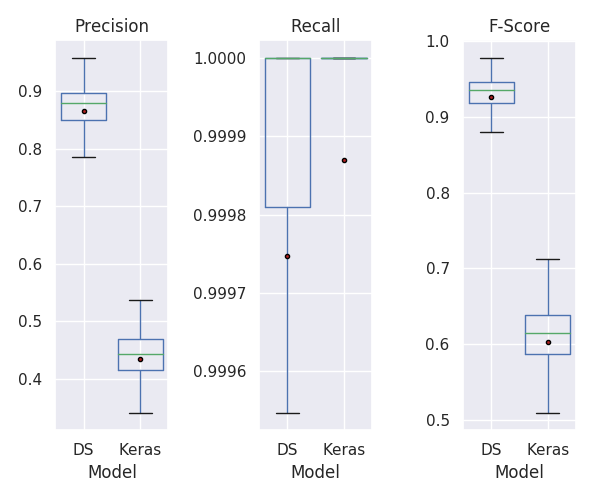
\includegraphics[width=3in]{boxplot_en.png}
		\caption{Precision, Recall and F-score of a pipeline using the Mozilla implementation of \textit{DeepSpeech} in its ASR stage compared against the same pipeline using the simplified model.}
		\label{boxplot_en}
	\end{center}
\end{figure}

\begin{table*}[h!]
	\centering
	\begin{tabular}{@{}rrrrcrrrcrrr@{}}
		\toprule
		& \multicolumn{2}{c}{$P$} & \phantom{abc} & \multicolumn{2}{c}{$R$} & \phantom{abc} & \multicolumn{2}{c}{$F$} \\
		\cmidrule{2-3} \cmidrule{5-6} \cmidrule{8-9} 
		& mean & median && mean & median && mean & median\\ 
		\midrule
		\textbf{Reference pipeline} & 0.865 & 0.879 && 0.999 & 1.0 && 0.926 & 0.935 \\
		\textbf{Simplified pipeline} & 0.435 & 0.443 && 0.999 & 1.0 && 0.602 & 0.614 \\
		\bottomrule
	\end{tabular}
	\caption{Average Precision ($P$), Recall ($R$) and F-Score ($F$) of alignments produced over all test samples for a pipeline using the reference model in the ASR stage compared to the results of the same pipeline using a simplified model}
	\label{prf_en}
\end{table*}

It is evident that $P$ and thus $F$ is significantly higher for the pipeline using the reference ASR model. This is no surprise because the transcript produced by the reference model are generally much better quality. However, $P$, $R$ and $F$ measure the quality of alignment for each pipeline in isolation. To capture the quality of alignments from the pipeline using the simplified model better, they were compared against the reference alignments produced by the pipeline using the pre-trained model from Mozilla. The latter is considered a hypothetical optimum and the comparison is made by calculating the average \textit{Levenshtein Similarity} between the alignments for each sample. Figure \ref{scatterplot_en} visualizes these values in a scatter plot.

\begin{figure}[!htb]
	\begin{center}
		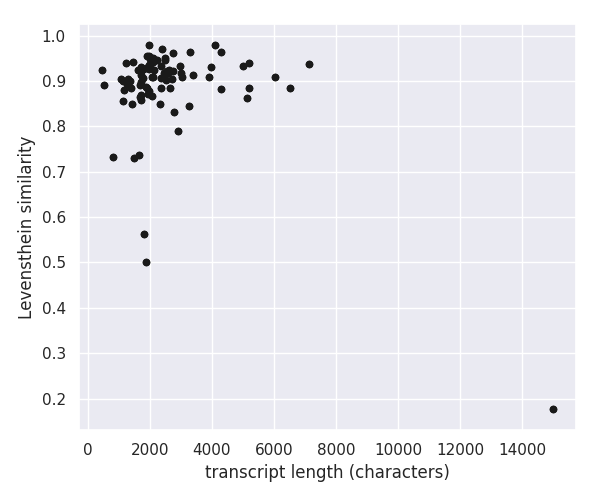
\includegraphics[width=3in]{scatterplot_en.png}
		\caption{Precision, Recall and F-score of a pipeline using the Mozilla implementation of \textit{DeepSpeech} in its ASR stage compared against the same pipeline using the simplified model.}
		\label{scatterplot_en}
	\end{center}
\end{figure}

Obviously the lower values of $P$ and $F$ for alignments produced by the pipeline using the simplified model did not affect the result very much. Alignemts produced by the pipeline using the simplified model are very similar to the ones produced with the pipeline using the reference model, with the average similarity ranging betwen 0.9 and 1.0 for most samples. This is true regardless of the length of the transcript with only a few outliers. This came a bit as a surprise. Obviously, the \textit{Needleman-Wunsch} algorithm can handle faulty partial transcripts very well and makes the alignments based on only few character sequences. The high quality of alignments produced by pipeline using the simplified model is justified when visualizing the alignment by highlighting the aligned text as the audio is being played. The perceived quality is then considered very high, with only few words at the beginning or end of an alignment being assigned the wrong voiced segment.

\section{Transfer to other languages}

Above tests were repeated with a pipeline using the simplified model trained on German samples (including synthesized data). The test set consisted of six short and 6 longer recordings of German speakers together with their transcripts. Because the split into training-, validation- and test-set was done automatically, all samples happen to be read by female speakers. Figure \ref{boxplot_de} contains the box plots for $P$, $R$ and $F$ calculated for the alignments produced by this pipeline. The values are very similar to the ones achieved on English samples. Obviously the change in language did not affect the result very much. This has to be taken with a pinch of salt however, because the distribution of the test set does not reflect a realistic scenario. It is also too small to draw generalizable conclusions from it.

\begin{figure}[!htb]
	\begin{center}
		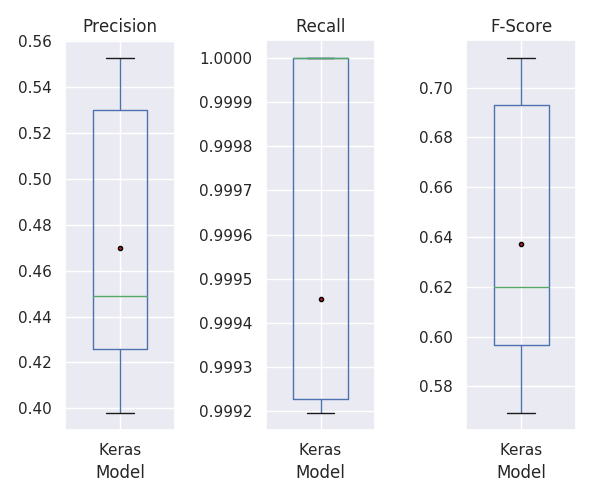
\includegraphics[width=3in]{boxplot_de.png}
		\caption{Precision, Recall and F-score of a pipeline using the simplified model that was trained on 1,000 minutes of German data (original and synthesized).}
		\label{boxplot_de}
	\end{center}
\end{figure}

Since there was no reference ASR model for German, the alignments could not be compared to reference alignments. Instead, they were compared to alignments derived from manual inspection. Figure \ref{scatterplot_de} shows the similarities between both alignments. It is evident that the shorter and longer samples form clusters in the plot. Apparently the similarity between alignments decreases for longer samples.

\begin{figure}[!htb]
	\begin{center}
		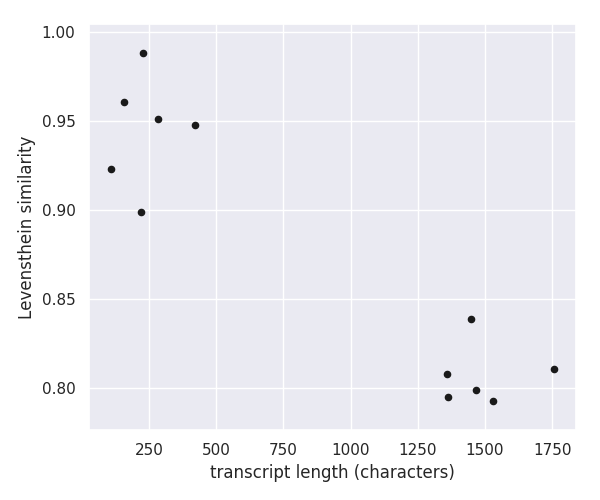
\includegraphics[width=3in]{scatterplot_de.png}
		\caption{Levenshein similarity between alignments produced by the pipeline using the simplified model and manually produced alignments. Note how the shorter and longer samples form clusters in the plot, while the alignments for the shorter samples are generally more similar to the manual alignments.}
		\label{scatterplot_de}
	\end{center}
\end{figure}

\section{Conclusion and further work}

Above results were made on English and German samples and might be valid for other languages as well. The pipeline approach generally works very well on these languages. However, it is expected to fail when being applied to samples of languages of other families. Such languages (e.g. Asian languages) can use completely different phonetic and/or graphological concepts. However the alignment produced by the pipeline might be considered a good starting point for many cases, needing only minor manual adjustments (sometimes even none).

Since the results for German samples were achieved with only 80 minutes of training data, they are promising for languages where labelled data is hard and/or expensive to acquire. Furthermore, for the alignments being a combination of audio/transcript, it would be interesting whether this pipeline could be used to generate labelled data to train a STT model, maybe even the one used in the pipeline.


\footnotesize
\printbibliography
%\bibliographystyle{apalike}
%\bibliography{mybib}


\end{document}